\documentclass{article}

% Language setting
\usepackage[polish]{babel}

% Set page size and margins
% Replace `letterpaper' with `a4paper' for UK/EU standard size
\usepackage[letterpaper,top=2cm,bottom=2cm,left=3cm,right=3cm,marginparwidth=1.75cm]{geometry}

% Useful packages
\usepackage{amsmath}
\usepackage{graphicx}
\usepackage[T1]{fontenc}
\usepackage[colorlinks=true, allcolors=blue]{hyperref}
\usepackage{lipsum}
\usepackage{multicol}
\usepackage{tikz,tcolorbox}
\usepackage{float}

\title{Metoda klasyfikacji cukierków na podstawie ich opakowania}
\author{Aleksander Golus, Bartosz Chadryś, Jakub Miśko, Igor Joński}

\begin{document}
\maketitle

\definecolor{my-red-light}{RGB}{254, 218, 212}
\definecolor{my-red-dark}{RGB}{220, 97, 85}
\definecolor{my-orange-light}{RGB}{252, 236, 189}
\definecolor{my-orange-dark}{RGB}{247, 167, 9}
\definecolor{my-pink-light}{RGB}{252, 218, 229}
\definecolor{my-pink-dark}{RGB}{247, 132, 168}
\definecolor{my-green}{RGB}{141, 189, 16}

\section{Wstęp}
\label{Wstęp}
W projekcie opracowano metodę, która pozwala na rozpoznawanie kolorowych opakowań cukierków oraz monitorowanie ich ilości na taśmie produkcyjnej. Metoda ta może znaleźć zastosowanie w przemyśle spożywczym w automatyzacji procesów pakowania oraz kontroli jakości. Zapewnia ona selekcję produktów oraz może przyczynić się do usprawnienia procesów magazynowania i dystrybucji.

Jednym z podobnych rozwiązań z tej branży (spożywczej) jest rozpoznawanie rodzajów bułek oraz ich kształtów tak jak zostało to przedstawione w \cite{virtuslab}, w przypadku tematu, jakim są cukierki, można znaleźć zastosowania w pomocy rozróżniania rodzaju cukierka w bombonierce \cite{chocolates}. Innym przypadkiem użycia detekcji obiektów na podstawie ich opakowania może być również przedstawiona tutaj \cite{vending} innowacyjna metoda rozpoznawania produktów w automatach sprzedających.

\section{Materiały i metody}
\label{Materiały i metody}
\subsection{Materiały badawcze}
\label{Materiały badawcze}
Materiałami badawczymi są konkretne rodzaje cukierków o kolorowych opakowaniach, to znaczy - cukierki marki Mamba oraz Turbo. Zostały one wybrane ze względu na to, że posiadają bardzo podobny rozmiar.

Wykorzystane cukierki dzielimy na 4 typy kolorów, z czego różowy, czerwony oraz pomarańczowy to cukierki marki Mamba, natomiast zielony - marki Turbo. Cukierki marki Mamba posiadają dwie barwy danego koloru - barwę jaśniejszą oraz ciemniejszą.

\begin{figure}[H]
    \centering
    \begin{tcolorbox}[colback=white]

    \begin{multicols}{4}
    Różowy cukierek
    \begin{tcolorbox}[colback=my-pink-dark, width=\linewidth, colframe=my-pink-dark]
    \end{tcolorbox}
    Czerwony cukierek
    \begin{tcolorbox}[colback=my-red-dark, width=\linewidth, colframe=my-red-dark]
    \end{tcolorbox}
    Pomarańczowy cuk.
    \begin{tcolorbox}[colback=my-orange-dark, width=\linewidth, colframe=my-orange-dark]
    \end{tcolorbox}
    Zielony cukierek
    \begin{tcolorbox}[colback=my-green, width=\linewidth, colframe=my-green]
    \end{tcolorbox}
    \end{multicols}

    \begin{multicols}{4}
    \begin{tcolorbox}[colback=my-pink-light, width=\linewidth, colframe=my-pink-light]
    \end{tcolorbox}
    \begin{tcolorbox}[colback=my-red-light, width=\linewidth, colframe=my-red-light]
    \end{tcolorbox}
    \begin{tcolorbox}[colback=my-orange-light, width=\linewidth, colframe=my-orange-light]
    \end{tcolorbox}
    \end{multicols}

    \end{tcolorbox}
    \caption{Wizualizacja barw dla każdego koloru badanego cukierka}
\end{figure}






\subsection{Przedziały kolorów rozpoznawalnych cukierków}

Kolory cukierków w określonym oświetleniu, omówionym w sekcji \ref{Układ pomiarowy}, powinny zawierać się w następujących zakresach:

\begin{table}[H]
    \label{tab:tab1}
    \centering
    \begin{tabular}{ |c|c|c|c| }
     \hline
     Kolor & Dolna granica & Górna granica \\
     \hline
     Różowy & \#32282f & \#ff0000 \\
     \hline
     Czerwony & \#645050 & \#ff7a37 \\
     \hline
     Pomarańczowy & \#644b3d & \#ffd500 \\
     \hline
     Zielony & \#323222 & \#00ff00 \\
     \hline
    \end{tabular}
    \caption{Przedziały barw, w których musi znaleźć się kolor opakowania cukierka by został zidentyfikowany.}
\end{table}

\subsection{Układ pomiarowy}
\label{Układ pomiarowy}

\begin{figure}[H]
    \centering
    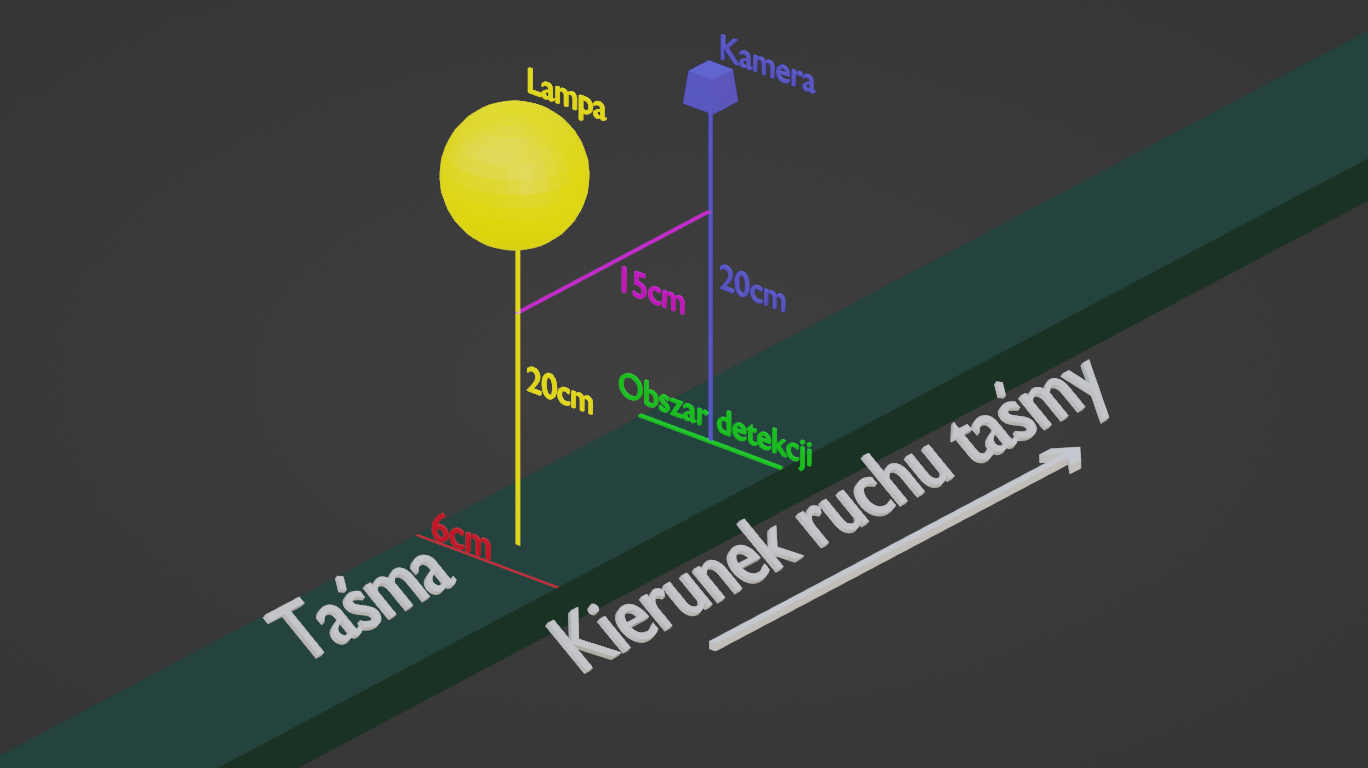
\includegraphics[width=\linewidth]{ukladPomiarowy.png}
    \caption{Układ pomiarowy}
    \label{fig:ukladPomiarowy}
\end{figure}

Układ pomiarowy, przedstawiony na rysunku \ref{fig:ukladPomiarowy}, składa się z ciemnozielonej taśmy produkcyjnej napędzanej silnikiem elektrycznym o stałej prędkości, kamery o rozdzielczości 1080p oraz lampy LED naświetlającej taśmę z góry. Ciemnozielony kolor taśmy został wybrany tak, aby nie zawierał się w przedziałach barw cukierków podanych w \ref{tab:tab1}.

Taśma produkcyjna ma szerokość 6cm, która przesuwa umieszczone na niej cukierki ze stałą prędkością 3cm/s. Do oświetlenia cukierków znajdujących się na taśmie została użyta lampa ledowa o mocy 10W i temperaturze 3500K, umieszczona na wysokości 20cm, oddalona od kamery o 15cm w płaszczyźnie poziomej. Kamera została ustawiona 20cm nad taśmą, rejestrując przy tym całą szerokość taśmy.

\subsection{Metoda pomiarowa}
\label{Metoda pomiarowa}
\subsubsection{Idea}
\label{Idea}

\begin{figure}[H]
    \centering
    \includegraphics[height=8cm]{diagram_idei.png}
    \caption{Diagram idei metody pomiarowej}
    \label{fig:diagramIdei}
\end{figure}

Ideą metody pomiarowej, przedstawionej na diagramie \ref{fig:diagramIdei}, jest zliczanie cukierków umieszczonych na taśmie produkcyjnej bazując na kolorze opakowania cukierka. Przypadki użycia metody pomiarowej to między innymi:

\begin{itemize}
    \item Weryfikacja ilości cukierków w partii - czy ilość zliczonych cukierków jest zgodna z ustaloną ilością w danej partii.
    \item Weryfikacja różnorodności cukierków - czy zliczone cukierki na taśmie są wystarczająco zróżnicowane.
\end{itemize}

\subsubsection{Sposób pomiaru}
\label{Sposób pomiaru}

Metoda została przedstawiona na diagramie \ref{}

\section{Wyniki i dyskusja}
\label{Wyniki i dyskusja}
Efektywność działania metody została przetestowana na dwóch wcześniej przygotowanych nagraniach taśmy produkcyjnej z umieszczonymi na niej cukierkami z których wyodrębniono przypadki.
\subsection{Przypadek 1}
Analizując rezultaty otrzymaliśmy następujące wyniki:

\begin{table}
\centering
\label{tab:video1}
\begin{tabular}{|p{0.15\linewidth}|p{0.25\linewidth}|p{0.25\linewidth}|p{0.25\linewidth}|}
 \hline
 Kolor opakowania & Rzeczywista ilość cukierków & Ilość cukierków rozpoznana przez metodę & Procent rozpoznanych cukierków \\
 \hline
 Czerwony & 4 & 4 & 100\% \\
 \hline
 Różowy & 6 & 6 & 100\% \\
 \hline
 Pomarańczowy & 8 & 8 & 100\% \\
 \hline
 Zielony & 7 & 7 & 100\% \\
 \hline
\end{tabular}
\caption{Wyniki dla pierwszego przypadku}
\end{table}

\begin{center}
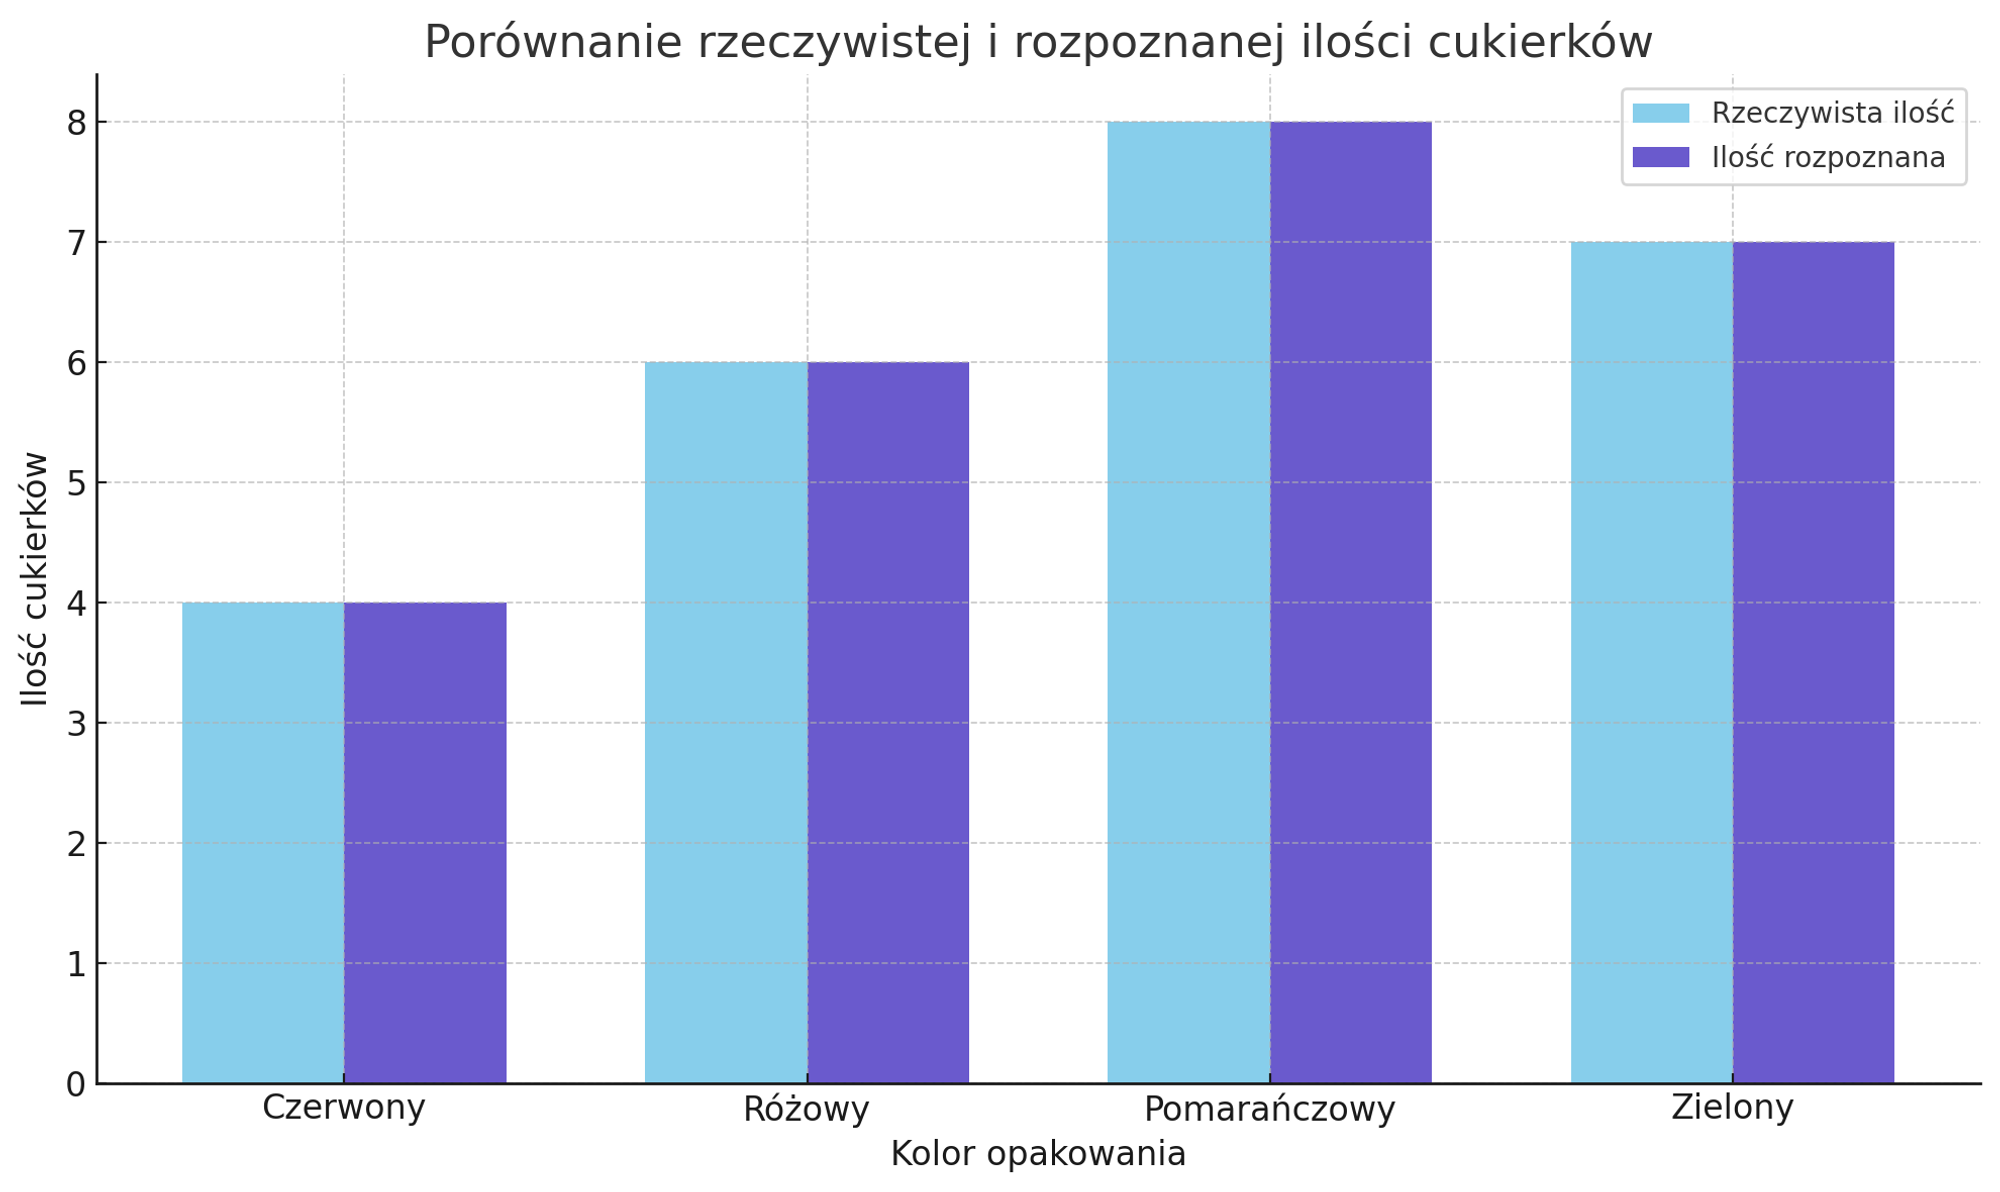
\includegraphics[width=\linewidth]{wykres1.png}
\end{center}

\begin{figure}[H]
    \centering
    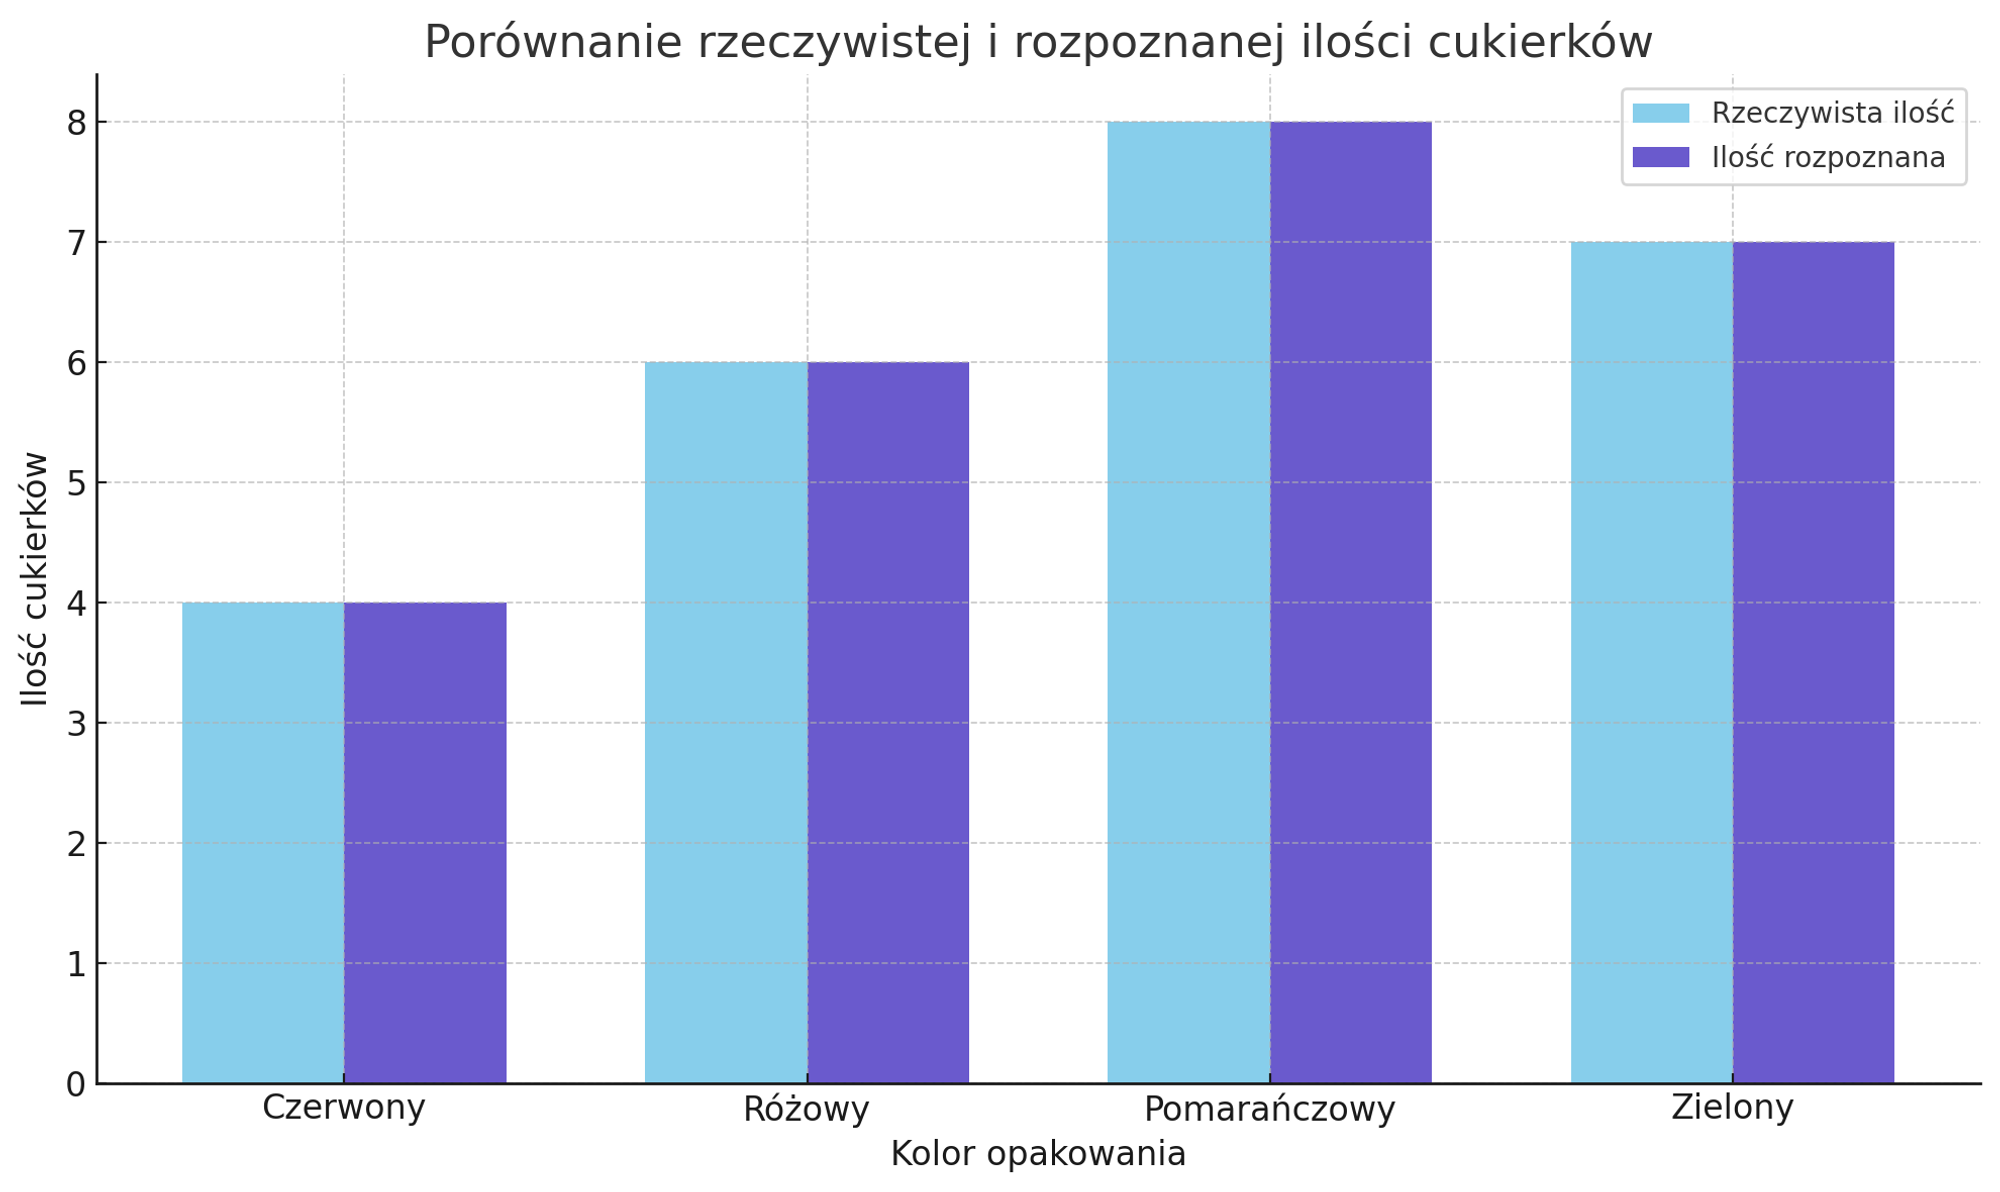
\includegraphics[width=\linewidth]{wykres1.png}
    \caption{Wykres rezultatów z pierwszego nagrania}
    \label{fig:ukladPomiarowy}
\end{figure}

Jak widać, nasza metoda dla nagrania 1. (który jest zgodny z wyżej wyjaśnioną konfiguracją stanowiska pomiarowego) daje wyniki 100-tu procentowej zgodności między rzeczywistą ilością cukierków, a tą rozpoznaną przez program, dla danego koloru opakowania cukierka.

Nagranie to pokazuje poprawne działanie metody, nawet w sytuacji, gdy na linii zliczającej kolor cukierka znajdują się jednocześnie dwa cukierki, jeden pod drugim.

\begin{center}
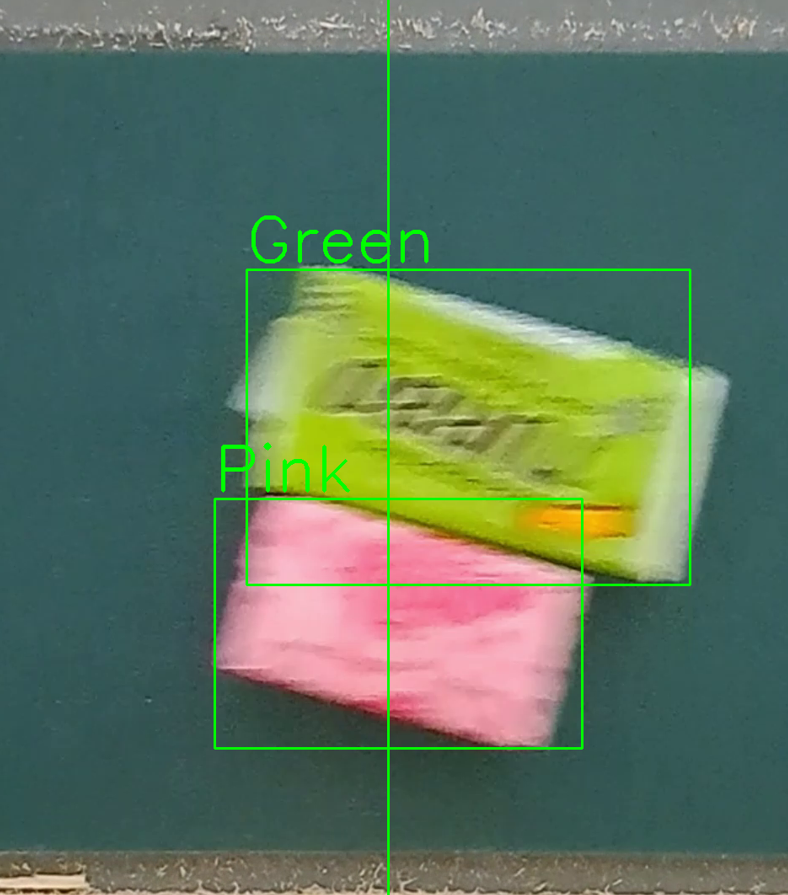
\includegraphics[width=6cm]{badanie.png}
\end{center}

\subsection{Nagranie 2}


\begin{center}
\begin{tabular}{|p{0.15\linewidth}|p{0.25\linewidth}|p{0.25\linewidth}|p{0.25\linewidth}|}
 \hline
 Kolor opakowania & Rzeczywista ilość cukierków & Ilość cukierków rozpoznana przez metodę & Procent rozpoznanych cukierków \\
 \hline
 Czerwony & 7 & 6 & 85\% \\
 \hline
 Różowy & 8 & 7 & 87\% \\
 \hline
 Pomarańczowy & 8 & 7 & 87\% \\
 \hline
 Zielony & - & - & -\% \\
 \hline
\end{tabular}
\end{center}

\begin{center}
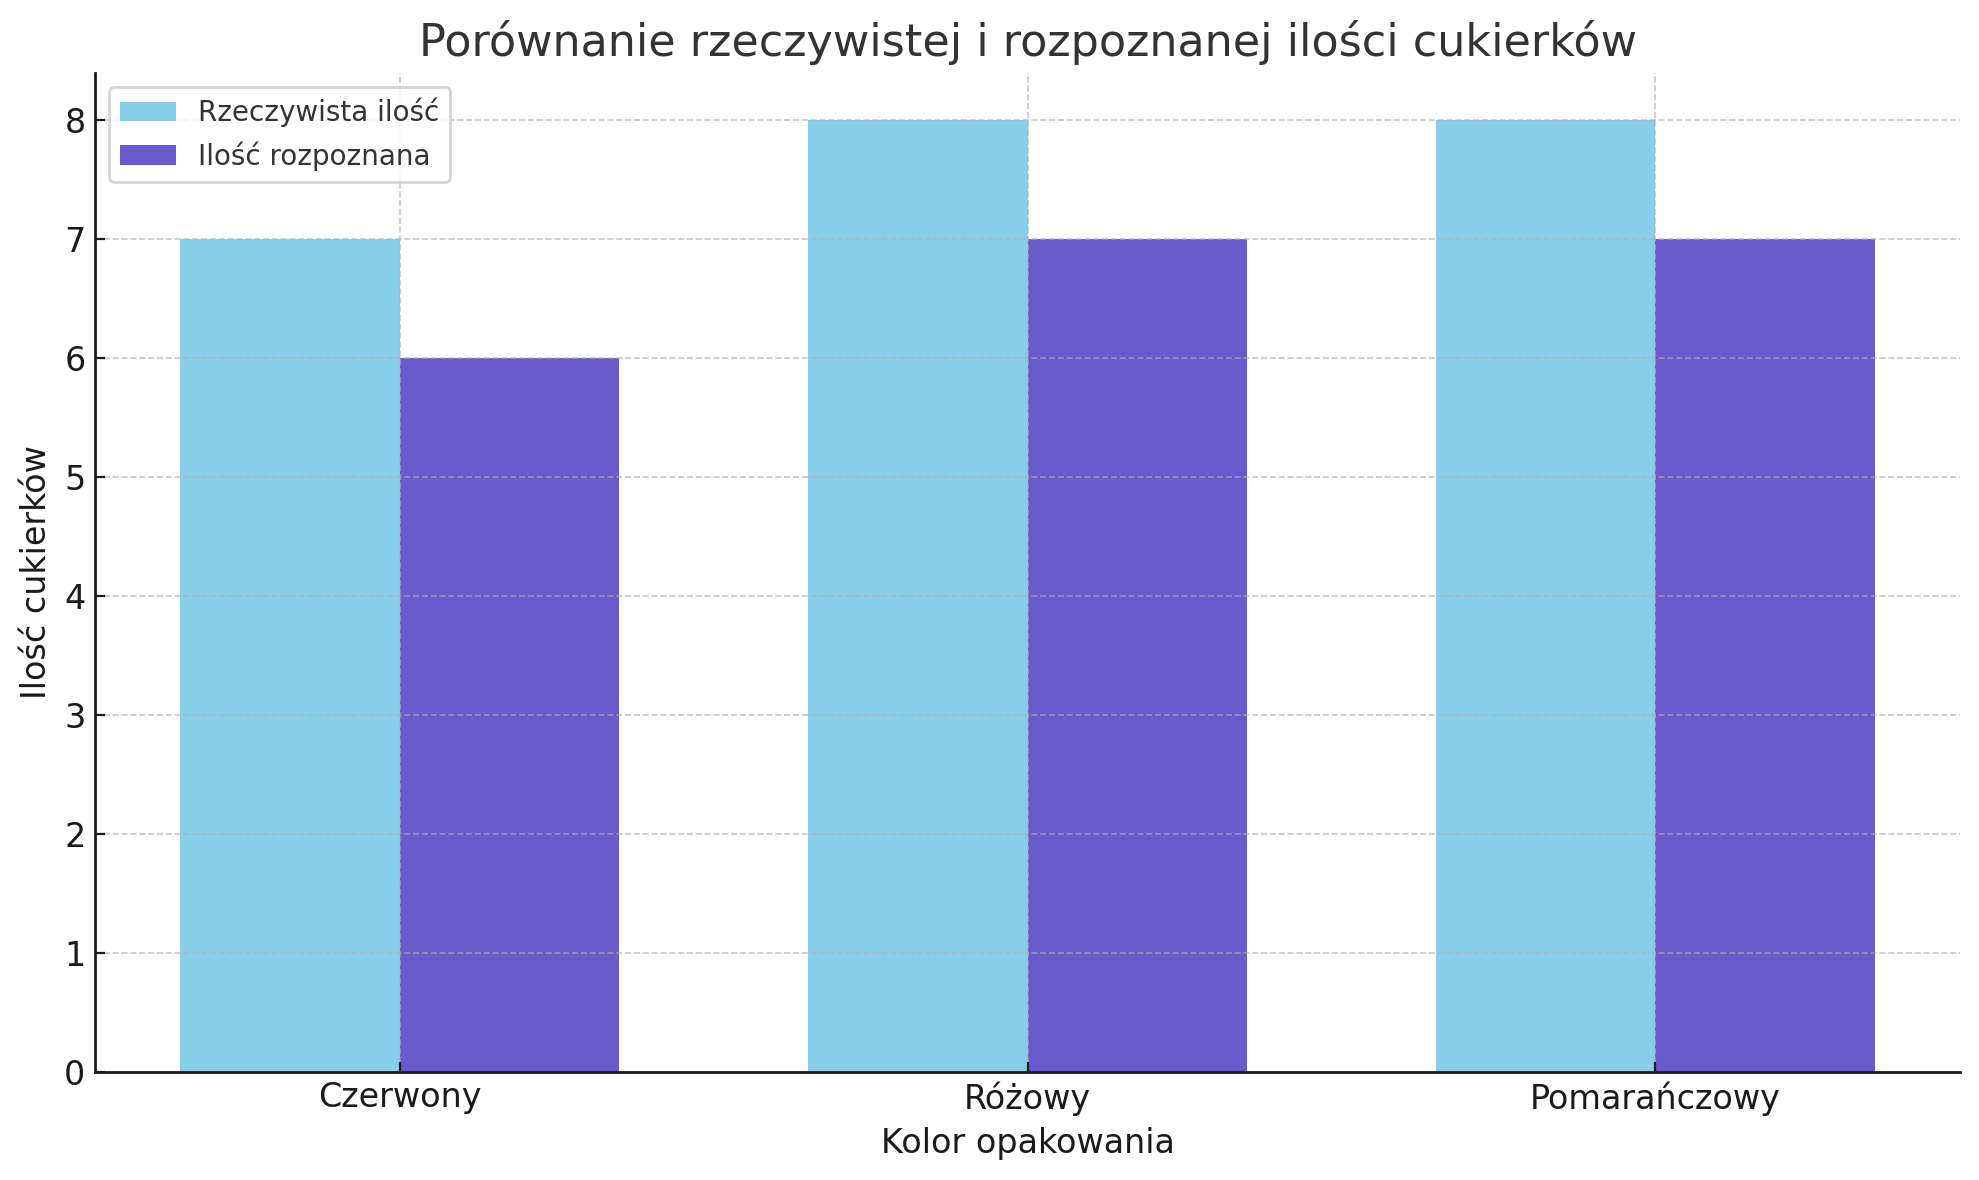
\includegraphics[width=\linewidth]{wykres2.png}
\end{center}

Nagranie 2. nie posiada żadnych cukierków o zielonym kolorze opakowania, więc zostały wyłączone z dyskusji na tym przykładzie.

Na tym nagraniu nasz program nie osiągnął 100\% w żadnym z obserwowanych kolorów. Niedokładność ta w każdym przypadku była spowodowana przez ten sam przypadek. Ponieważ nasza metoda klasyfikuje cukierek tylko na podstawie jego koloru, program ma problem z rozpoznaniem dwóch cukierków tego samego koloru znajdujących się bezpośrednio obok siebie (stykających się ze sobą). Na nagraniu 1. przypadek ten nie wystąpił, stąd otrzymaliśmy początkowo idealną dokładność.

\begin{center}
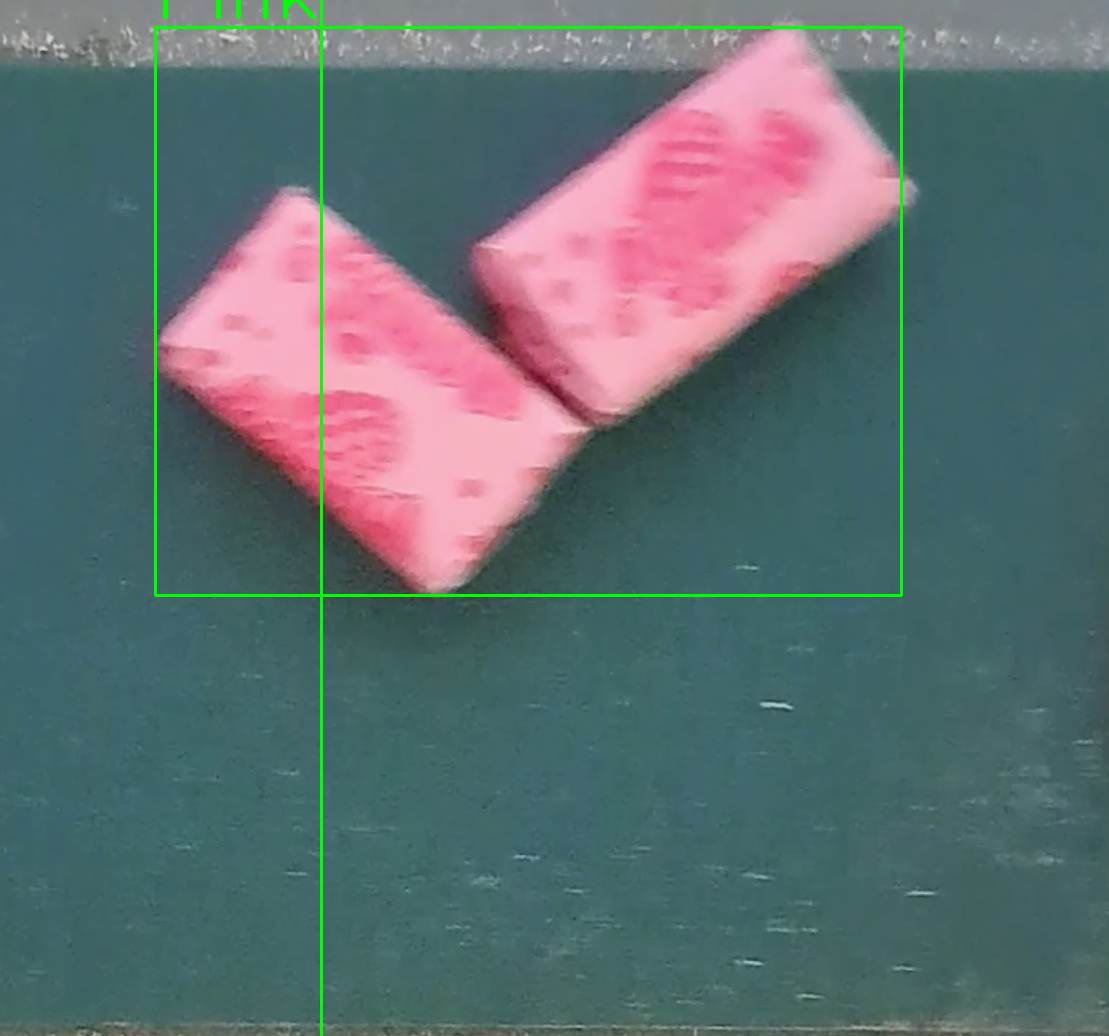
\includegraphics[width=0.3\linewidth]{pink.png}
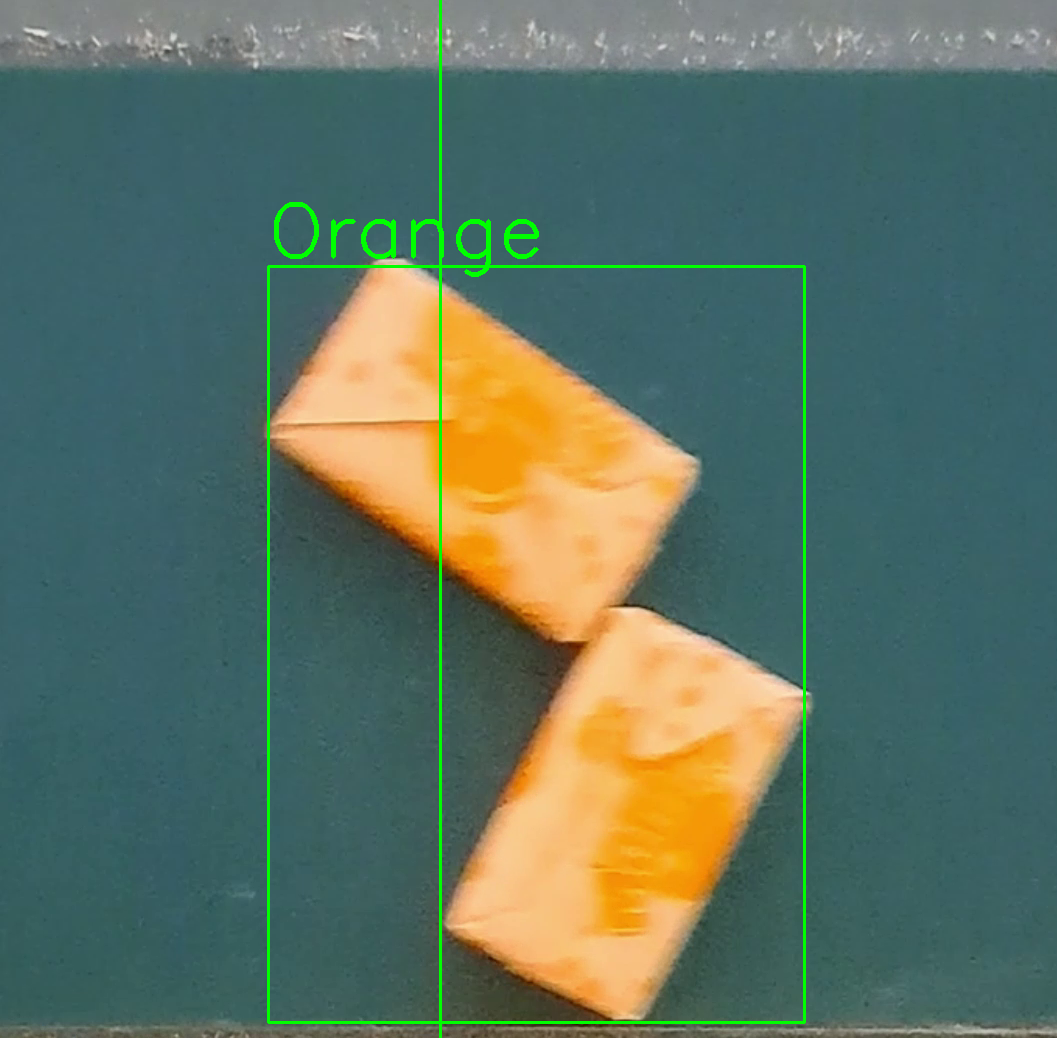
\includegraphics[width=0.3\linewidth]{orange.png}
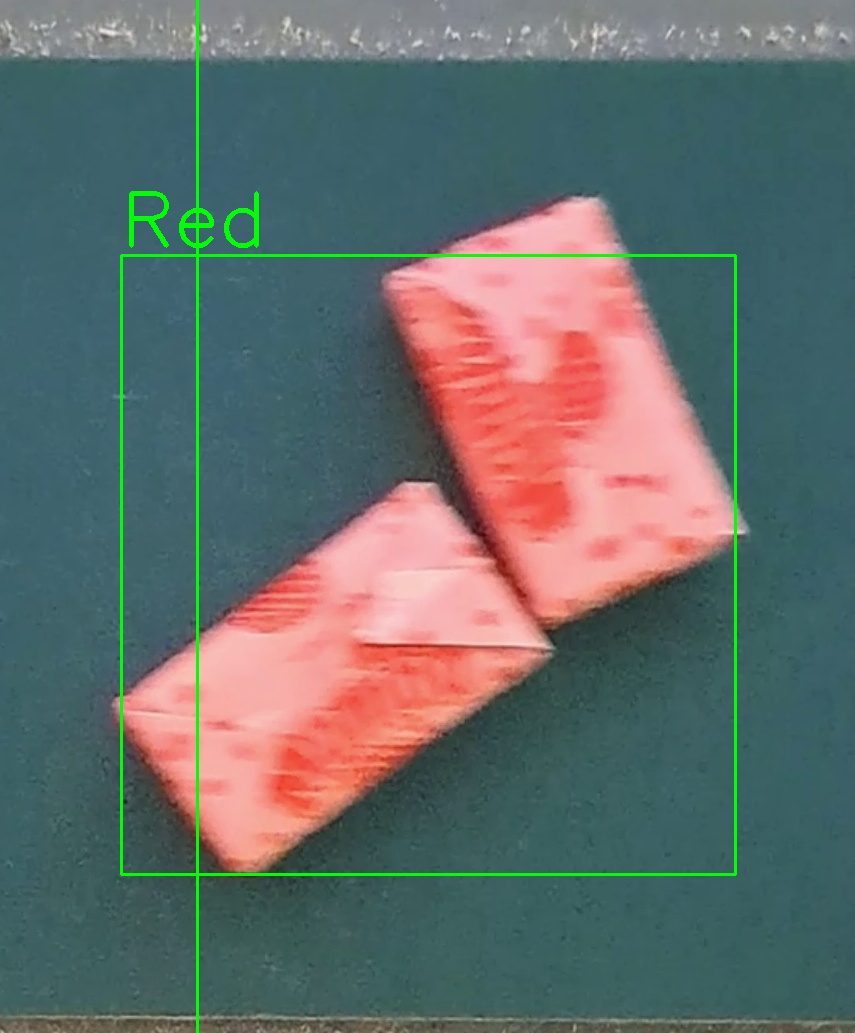
\includegraphics[width=0.3\linewidth]{red.png}
\end{center}

\subsection{Skuteczność metody na podstawie obu nagrań}

Łącznie na obu nagraniach wystąpiło 48 cukierków, z czego poprawnie rozpoznano 45 z nich. Daje nam to średnią dokładność 94\%. Aby otrzymać jak najlepsze wyniki warto zadbać o różnorodność kolorów opakowań cukierkó na taśmie znajdujących się bezpośrednio nad czytnikiem w danej chwili.

\section{Wnioski}
\label{Wnioski}

Metoda została zaprojektowana w celu zliczania ilości cukierków na podstawie koloru ich opakowań na nagraniu. Uzyskane wyniki były zgodne z założeniami projektu. Skuteczność rozpoznawania cukierków po opakowaniach wynosiła 94\%, a precyzja wahała się w granicach +/- 2 cukierki.

Analiza dokładności rozwiązania wykazała, że system skutecznie identyfikuje cukierki o różnych kolorach dla określonego rozmiaru minimalnego.

Podczas działania programu zostaje wykorzystywane około 200MB pamięci RAM. Jednakże większe zużycie zasobów wystąpiło na procesorze 30\% - 45\% mocy obliczeniowej. Nie wpłynęło to w żaden sposób na pracę komputera ani programu, nie wystąpiły spowolnienia systemu, a program działał bez żadnych spowolnień ani błędów.

Rozwiązanie to możne znaleźć zastosowanie w branży spożywczej do zliczania ilości cukierków.

\section{Literatura}
\label{Literatura}
\begin{thebibliography}{9}

\bibitem{opencv1}
\url{https://docs.opencv.org/3.4/d8/dfe/classcv_1_1VideoCapture.html#a949d90b766ba42a6a93fe23a67785951}

\bibitem{opencv2}
\url{https://docs.opencv.org/3.4/d8/dfe/classcv_1_1VideoCapture.html#a9d2ca36789e7fcfe7a7be3b328038585}

\bibitem{opencv3}
\url{https://docs.opencv.org/3.4/d8/dfe/classcv_1_1VideoCapture.html#a473055e77dd7faa4d26d686226b292c1}

\bibitem{opencv4}
\url{https://docs.opencv.org/3.4/d8/d01/group__imgproc__color__conversions.html#ga397ae87e1288a81d2363b61574eb8cab}

\bibitem{opencv5}
\url{https://docs.opencv.org/3.4/d7/dfc/group__highgui.html#ga453d42fe4cb60e5723281a89973ee563}

\bibitem{opencv6}
\url{https://docs.opencv.org/3.4/d7/dfc/group__highgui.html#ga5628525ad33f52eab17feebcfba38bd7}

\bibitem{opencv7}
\url{https://docs.opencv.org/3.4/d6/d6e/group__imgproc__draw.html#ga5126f47f883d730f633d74f07456c576}

\bibitem{opencv8}
\url{https://docs.opencv.org/3.4/d3/dc0/group__imgproc__shape.html#ga17ed9f5d79ae97bd4c7cf18403e1689a}

\bibitem{opencv9}
\url{https://docs.opencv.org/3.4/d3/dc0/group__imgproc__shape.html#ga2c759ed9f497d4a618048a2f56dc97f1}

\bibitem{opencv10}
\url{https://docs.opencv.org/3.4/d3/dc0/group__imgproc__shape.html#ga103fcbda2f540f3ef1c042d6a9b35ac7}

\bibitem{opencv11}
\url{https://docs.opencv.org/3.4/d2/de8/group__core__array.html#ga48af0ab51e36436c5d04340e036ce981}

\bibitem{opencv12}
\url{https://docs.opencv.org/3.4/d6/d6e/group__imgproc__draw.html#ga07d2f74cadcf8e305e810ce8eed13bc9}

\bibitem{opencv13}
\url{https://docs.opencv.org/3.4/d8/dfe/classcv_1_1VideoCapture.html#afb4ab689e553ba2c8f0fec41b9344ae6}

\bibitem{opencv14}
\url{https://docs.opencv.org/3.4/d7/dfc/group__highgui.html#ga6b7fc1c1a8960438156912027b38f481}

\bibitem{opencv15}
\url{https://docs.opencv.org/3.4/d7/d1b/group__imgproc__misc.html#gae8a4a146d1ca78c626a53577199e9c57}

\bibitem{opencv16}
\url{https://docs.opencv.org/3.4/d6/d6e/group__imgproc__draw.html#ga7078a9fae8c7e7d13d24dac2520ae4a2}

\bibitem{virtuslab}
\url{https://virtuslab.com/case-study/object-detection-in-real-time-streaming-recordings-and-images}

\bibitem{gfg}
\url{https://www.geeksforgeeks.org/detect-an-object-with-opencv-python/}

\bibitem{dry}
\url{https://dontrepeatyourself.org/post/color-based-object-detection-with-opencv-and-python/}

\bibitem{yt-motorcycle}
\url{https://www.youtube.com/watch?v=O3b8lVF93jU/}

\bibitem{yt-banana}
\url{https://www.youtube.com/watch?v=aFNDh5k3SjU&t=1004s/}

\bibitem{chocolates}
\url{https://blog.roboflow.com/identifying-chocolates-with-computer-vision/}

\bibitem{vending}
 \url{https://www.researchgate.net/publication/337068624_Towards_Identification_of_Packaged_Products_via_Computer_Vision_Convolutional_Neural_Networks_for_Object_Detection_and_Image_Classification_in_Retail_Environments}

\end{thebibliography}

\end{document}